\documentclass[1p]{elsarticle_modified}
%\bibliographystyle{elsarticle-num}

%\usepackage[colorlinks]{hyperref}
%\usepackage{abbrmath_seonhwa} %\Abb, \Ascr, \Acal ,\Abf, \Afrak
\usepackage{amsfonts}
\usepackage{amssymb}
\usepackage{amsmath}
\usepackage{amsthm}
\usepackage{scalefnt}
\usepackage{amsbsy}
\usepackage{kotex}
\usepackage{caption}
\usepackage{subfig}
\usepackage{color}
\usepackage{graphicx}
\usepackage{xcolor} %% white, black, red, green, blue, cyan, magenta, yellow
\usepackage{float}
\usepackage{setspace}
\usepackage{hyperref}

\usepackage{tikz}
\usetikzlibrary{arrows}

\usepackage{multirow}
\usepackage{array} % fixed length table
\usepackage{hhline}

%%%%%%%%%%%%%%%%%%%%%
\makeatletter
\renewcommand*\env@matrix[1][\arraystretch]{%
	\edef\arraystretch{#1}%
	\hskip -\arraycolsep
	\let\@ifnextchar\new@ifnextchar
	\array{*\c@MaxMatrixCols c}}
\makeatother %https://tex.stackexchange.com/questions/14071/how-can-i-increase-the-line-spacing-in-a-matrix
%%%%%%%%%%%%%%%

\usepackage[normalem]{ulem}

\newcommand{\msout}[1]{\ifmmode\text{\sout{\ensuremath{#1}}}\else\sout{#1}\fi}
%SOURCE: \msout is \stkout macro in https://tex.stackexchange.com/questions/20609/strikeout-in-math-mode

\newcommand{\cancel}[1]{
	\ifmmode
	{\color{red}\msout{#1}}
	\else
	{\color{red}\sout{#1}}
	\fi
}

\newcommand{\add}[1]{
	{\color{blue}\uwave{#1}}
}

\newcommand{\replace}[2]{
	\ifmmode
	{\color{red}\msout{#1}}{\color{blue}\uwave{#2}}
	\else
	{\color{red}\sout{#1}}{\color{blue}\uwave{#2}}
	\fi
}

\newcommand{\Sol}{\mathcal{S}} %segment
\newcommand{\D}{D} %diagram
\newcommand{\A}{\mathcal{A}} %arc


%%%%%%%%%%%%%%%%%%%%%%%%%%%%%5 test

\def\sl{\operatorname{\textup{SL}}(2,\Cbb)}
\def\psl{\operatorname{\textup{PSL}}(2,\Cbb)}
\def\quan{\mkern 1mu \triangleright \mkern 1mu}

\theoremstyle{definition}
\newtheorem{thm}{Theorem}[section]
\newtheorem{prop}[thm]{Proposition}
\newtheorem{lem}[thm]{Lemma}
\newtheorem{ques}[thm]{Question}
\newtheorem{cor}[thm]{Corollary}
\newtheorem{defn}[thm]{Definition}
\newtheorem{exam}[thm]{Example}
\newtheorem{rmk}[thm]{Remark}
\newtheorem{alg}[thm]{Algorithm}

\newcommand{\I}{\sqrt{-1}}
\begin{document}

%\begin{frontmatter}
%
%\title{Boundary parabolic representations of knots up to 8 crossings}
%
%%% Group authors per affiliation:
%\author{Yunhi Cho} 
%\address{Department of Mathematics, University of Seoul, Seoul, Korea}
%\ead{yhcho@uos.ac.kr}
%
%
%\author{Seonhwa Kim} %\fnref{s_kim}}
%\address{Center for Geometry and Physics, Institute for Basic Science, Pohang, 37673, Korea}
%\ead{ryeona17@ibs.re.kr}
%
%\author{Hyuk Kim}
%\address{Department of Mathematical Sciences, Seoul National University, Seoul 08826, Korea}
%\ead{hyukkim@snu.ac.kr}
%
%\author{Seokbeom Yoon}
%\address{Department of Mathematical Sciences, Seoul National University, Seoul, 08826,  Korea}
%\ead{sbyoon15@snu.ac.kr}
%
%\begin{abstract}
%We find all boundary parabolic representation of knots up to 8 crossings.
%
%\end{abstract}
%\begin{keyword}
%    \MSC[2010] 57M25 
%\end{keyword}
%
%\end{frontmatter}

%\linenumbers
%\tableofcontents
%
\newcommand\colored[1]{\textcolor{white}{\rule[-0.35ex]{0.8em}{1.4ex}}\kern-0.8em\color{red} #1}%
%\newcommand\colored[1]{\textcolor{white}{ #1}\kern-2.17ex	\textcolor{white}{ #1}\kern-1.81ex	\textcolor{white}{ #1}\kern-2.15ex\color{red}#1	}

{\Large $\underline{12a_{0415}~(K12a_{0415})}$}

\setlength{\tabcolsep}{10pt}
\renewcommand{\arraystretch}{1.6}
\vspace{1cm}\begin{tabular}{m{100pt}>{\centering\arraybackslash}m{274pt}}
\multirow{5}{120pt}{
	\centering
	\includegraphics[width=112pt]{../../../GIT/diagram.site/Diagrams/png/1216_12a_0415.png}\\
\ \ \ A knot diagram\footnotemark}&
\allowdisplaybreaks
\textbf{Linearized knot diagam} \\
\cline{2-2}
 &
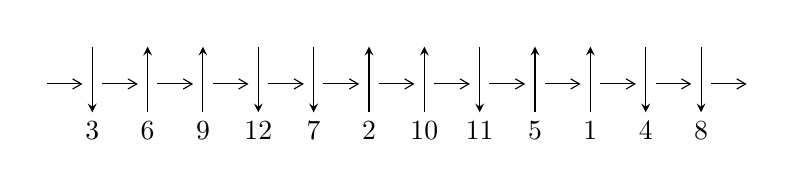
\begin{tikzpicture}[x=20pt, y=17pt]
	% nodes
	\node (C0) at (0, 0) {};
	\node (C1) at (1, 0) {};
	\node (C1U) at (1, +1) {};
	\node (C1D) at (1, -1) {3};

	\node (C2) at (2, 0) {};
	\node (C2U) at (2, +1) {};
	\node (C2D) at (2, -1) {6};

	\node (C3) at (3, 0) {};
	\node (C3U) at (3, +1) {};
	\node (C3D) at (3, -1) {9};

	\node (C4) at (4, 0) {};
	\node (C4U) at (4, +1) {};
	\node (C4D) at (4, -1) {12};

	\node (C5) at (5, 0) {};
	\node (C5U) at (5, +1) {};
	\node (C5D) at (5, -1) {7};

	\node (C6) at (6, 0) {};
	\node (C6U) at (6, +1) {};
	\node (C6D) at (6, -1) {2};

	\node (C7) at (7, 0) {};
	\node (C7U) at (7, +1) {};
	\node (C7D) at (7, -1) {10};

	\node (C8) at (8, 0) {};
	\node (C8U) at (8, +1) {};
	\node (C8D) at (8, -1) {11};

	\node (C9) at (9, 0) {};
	\node (C9U) at (9, +1) {};
	\node (C9D) at (9, -1) {5};

	\node (C10) at (10, 0) {};
	\node (C10U) at (10, +1) {};
	\node (C10D) at (10, -1) {1};

	\node (C11) at (11, 0) {};
	\node (C11U) at (11, +1) {};
	\node (C11D) at (11, -1) {4};

	\node (C12) at (12, 0) {};
	\node (C12U) at (12, +1) {};
	\node (C12D) at (12, -1) {8};
	\node (C13) at (13, 0) {};

	% arrows
	\draw[->,>={angle 60}]
	(C0) edge (C1) (C1) edge (C2) (C2) edge (C3) (C3) edge (C4) (C4) edge (C5) (C5) edge (C6) (C6) edge (C7) (C7) edge (C8) (C8) edge (C9) (C9) edge (C10) (C10) edge (C11) (C11) edge (C12) (C12) edge (C13) ;	\draw[->,>=stealth]
	(C1U) edge (C1D) (C2D) edge (C2U) (C3D) edge (C3U) (C4U) edge (C4D) (C5U) edge (C5D) (C6D) edge (C6U) (C7D) edge (C7U) (C8U) edge (C8D) (C9D) edge (C9U) (C10D) edge (C10U) (C11U) edge (C11D) (C12U) edge (C12D) ;
	\end{tikzpicture} \\
\hhline{~~} \\& 
\textbf{Solving Sequence} \\ \cline{2-2} 
 &
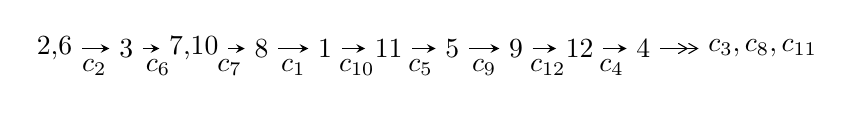
\begin{tikzpicture}[x=23pt, y=7pt]
	% node
	\node (A0) at (-1/8, 0) {2,6};
	\node (A1) at (1, 0) {3};
	\node (A2) at (33/16, 0) {7,10};
	\node (A3) at (25/8, 0) {8};
	\node (A4) at (33/8, 0) {1};
	\node (A5) at (41/8, 0) {11};
	\node (A6) at (49/8, 0) {5};
	\node (A7) at (57/8, 0) {9};
	\node (A8) at (65/8, 0) {12};
	\node (A9) at (73/8, 0) {4};
	\node (C1) at (1/2, -1) {$c_{2}$};
	\node (C2) at (3/2, -1) {$c_{6}$};
	\node (C3) at (21/8, -1) {$c_{7}$};
	\node (C4) at (29/8, -1) {$c_{1}$};
	\node (C5) at (37/8, -1) {$c_{10}$};
	\node (C6) at (45/8, -1) {$c_{5}$};
	\node (C7) at (53/8, -1) {$c_{9}$};
	\node (C8) at (61/8, -1) {$c_{12}$};
	\node (C9) at (69/8, -1) {$c_{4}$};
	\node (A10) at (11, 0) {$c_{3},c_{8},c_{11}$};

	% edge
	\draw[->,>=stealth]	
	(A0) edge (A1) (A1) edge (A2) (A2) edge (A3) (A3) edge (A4) (A4) edge (A5) (A5) edge (A6) (A6) edge (A7) (A7) edge (A8) (A8) edge (A9) ;
	\draw[->>,>={angle 60}]	
	(A9) edge (A10);
\end{tikzpicture} \\ 

\end{tabular} \\

\footnotetext{
The image of knot diagram is generated by the software ``\textbf{Draw programme}" developed by Andrew Bartholomew(\url{http://www.layer8.co.uk/maths/draw/index.htm\#Running-draw}), where we modified some parts for our purpose(\url{https://github.com/CATsTAILs/LinksPainter}).
}\phantom \\ \newline 
\centering \textbf{Ideals for irreducible components\footnotemark of $X_{\text{par}}$} 
 
\begin{align*}
I^u_{1}&=\langle 
-7.22695\times10^{232} u^{156}-2.83942\times10^{233} u^{155}+\cdots+7.03858\times10^{232} b-6.42788\times10^{232},\\
\phantom{I^u_{1}}&\phantom{= \langle  }-2.77552\times10^{233} u^{156}-1.00711\times10^{234} u^{155}+\cdots+7.03858\times10^{232} a-8.46264\times10^{233},\\
\phantom{I^u_{1}}&\phantom{= \langle  }u^{157}+3 u^{156}+\cdots+20 u-1\rangle \\
I^u_{2}&=\langle 
6 u^{32}-8 u^{31}+\cdots+b+3,\;u^{31}-4 u^{30}+\cdots+a+1,\;u^{33}-2 u^{32}+\cdots-2 u-1\rangle \\
\\
\end{align*}
\raggedright * 2 irreducible components of $\dim_{\mathbb{C}}=0$, with total 190 representations.\\
\footnotetext{All coefficients of polynomials are rational numbers. But the coefficients are sometimes approximated in decimal forms when there is not enough margin.}
\newpage
\renewcommand{\arraystretch}{1}
\centering \section*{I. $I^u_{1}= \langle -7.23\times10^{232} u^{156}-2.84\times10^{233} u^{155}+\cdots+7.04\times10^{232} b-6.43\times10^{232},\;-2.78\times10^{233} u^{156}-1.01\times10^{234} u^{155}+\cdots+7.04\times10^{232} a-8.46\times10^{233},\;u^{157}+3 u^{156}+\cdots+20 u-1 \rangle$}
\flushleft \textbf{(i) Arc colorings}\\
\begin{tabular}{m{7pt} m{180pt} m{7pt} m{180pt} }
\flushright $a_{2}=$&$\begin{pmatrix}1\\0\end{pmatrix}$ \\
\flushright $a_{6}=$&$\begin{pmatrix}0\\u\end{pmatrix}$ \\
\flushright $a_{3}=$&$\begin{pmatrix}1\\- u^2\end{pmatrix}$ \\
\flushright $a_{7}=$&$\begin{pmatrix}u\\u\end{pmatrix}$ \\
\flushright $a_{10}=$&$\begin{pmatrix}3.94330 u^{156}+14.3084 u^{155}+\cdots-215.833 u+12.0232\\1.02676 u^{156}+4.03408 u^{155}+\cdots+7.45787 u+0.913236\end{pmatrix}$ \\
\flushright $a_{8}=$&$\begin{pmatrix}-4.91003 u^{156}-11.8337 u^{155}+\cdots+405.512 u-35.1552\\-0.0408320 u^{156}+1.65797 u^{155}+\cdots+25.4097 u-1.67370\end{pmatrix}$ \\
\flushright $a_{1}=$&$\begin{pmatrix}u^2+1\\- u^4\end{pmatrix}$ \\
\flushright $a_{11}=$&$\begin{pmatrix}3.72168 u^{156}+14.4412 u^{155}+\cdots-240.641 u+14.6185\\-0.0679406 u^{156}+0.144116 u^{155}+\cdots-22.1587 u+2.44123\end{pmatrix}$ \\
\flushright $a_{5}=$&$\begin{pmatrix}u^3\\u^3+u\end{pmatrix}$ \\
\flushright $a_{9}=$&$\begin{pmatrix}3.94427 u^{156}+15.7459 u^{155}+\cdots-194.196 u+10.9237\\0.675606 u^{156}+3.31577 u^{155}+\cdots-6.23214 u+1.75659\end{pmatrix}$ \\
\flushright $a_{12}=$&$\begin{pmatrix}0.865828 u^{156}+3.51473 u^{155}+\cdots+134.531 u-19.8156\\1.78361 u^{156}+6.57450 u^{155}+\cdots-9.63089 u+0.852523\end{pmatrix}$ \\
\flushright $a_{4}=$&$\begin{pmatrix}-1.38787 u^{156}-3.84467 u^{155}+\cdots+22.3222 u+11.7347\\0.0715685 u^{156}+2.04385 u^{155}+\cdots+73.2958 u-4.75087\end{pmatrix}$\\&\end{tabular}
\flushleft \textbf{(ii) Obstruction class $= -1$}\\~\\
\flushleft \textbf{(iii) Cusp Shapes $= -7.48606 u^{156}-19.1787 u^{155}+\cdots+332.793 u-21.7130$}\\~\\
\newpage\renewcommand{\arraystretch}{1}
\flushleft \textbf{(iv) u-Polynomials at the component}\newline \\
\begin{tabular}{m{50pt}|m{274pt}}
Crossings & \hspace{64pt}u-Polynomials at each crossing \\
\hline $$\begin{aligned}c_{1},c_{5}\end{aligned}$$&$\begin{aligned}
&u^{157}+49 u^{156}+\cdots+66 u-1
\end{aligned}$\\
\hline $$\begin{aligned}c_{2},c_{6}\end{aligned}$$&$\begin{aligned}
&u^{157}-3 u^{156}+\cdots+20 u+1
\end{aligned}$\\
\hline $$\begin{aligned}c_{3}\end{aligned}$$&$\begin{aligned}
&u^{157}+u^{156}+\cdots+15730067 u+2315629
\end{aligned}$\\
\hline $$\begin{aligned}c_{4},c_{11}\end{aligned}$$&$\begin{aligned}
&u^{157}+u^{156}+\cdots+427 u+286
\end{aligned}$\\
\hline $$\begin{aligned}c_{7}\end{aligned}$$&$\begin{aligned}
&u^{157}-6 u^{156}+\cdots-586611 u-71082
\end{aligned}$\\
\hline $$\begin{aligned}c_{8}\end{aligned}$$&$\begin{aligned}
&u^{157}+7 u^{156}+\cdots-141270 u-7225
\end{aligned}$\\
\hline $$\begin{aligned}c_{9}\end{aligned}$$&$\begin{aligned}
&u^{157}+u^{156}+\cdots-1890458 u-514883
\end{aligned}$\\
\hline $$\begin{aligned}c_{10}\end{aligned}$$&$\begin{aligned}
&u^{157}+16 u^{156}+\cdots+71 u+1
\end{aligned}$\\
\hline $$\begin{aligned}c_{12}\end{aligned}$$&$\begin{aligned}
&u^{157}+8 u^{156}+\cdots-61 u+1
\end{aligned}$\\
\hline
\end{tabular}\\~\\
\newpage\renewcommand{\arraystretch}{1}
\flushleft \textbf{(v) Riley Polynomials at the component}\newline \\
\begin{tabular}{m{50pt}|m{274pt}}
Crossings & \hspace{64pt}Riley Polynomials at each crossing \\
\hline $$\begin{aligned}c_{1},c_{5}\end{aligned}$$&$\begin{aligned}
&y^{157}+125 y^{156}+\cdots-3938 y-1
\end{aligned}$\\
\hline $$\begin{aligned}c_{2},c_{6}\end{aligned}$$&$\begin{aligned}
&y^{157}+49 y^{156}+\cdots+66 y-1
\end{aligned}$\\
\hline $$\begin{aligned}c_{3}\end{aligned}$$&$\begin{aligned}
&y^{157}+17 y^{156}+\cdots-194381535859813 y-5362137665641
\end{aligned}$\\
\hline $$\begin{aligned}c_{4},c_{11}\end{aligned}$$&$\begin{aligned}
&y^{157}-93 y^{156}+\cdots+2756329 y-81796
\end{aligned}$\\
\hline $$\begin{aligned}c_{7}\end{aligned}$$&$\begin{aligned}
&y^{157}-34 y^{156}+\cdots-162359863767 y-5052650724
\end{aligned}$\\
\hline $$\begin{aligned}c_{8}\end{aligned}$$&$\begin{aligned}
&y^{157}-29 y^{156}+\cdots+11092528050 y-52200625
\end{aligned}$\\
\hline $$\begin{aligned}c_{9}\end{aligned}$$&$\begin{aligned}
&y^{157}-23 y^{156}+\cdots-20454032272420 y-265104503689
\end{aligned}$\\
\hline $$\begin{aligned}c_{10}\end{aligned}$$&$\begin{aligned}
&y^{157}-20 y^{156}+\cdots+353 y-1
\end{aligned}$\\
\hline $$\begin{aligned}c_{12}\end{aligned}$$&$\begin{aligned}
&y^{157}-14 y^{156}+\cdots+135 y-1
\end{aligned}$\\
\hline
\end{tabular}\\~\\
\newpage\flushleft \textbf{(vi) Complex Volumes and Cusp Shapes}
$$\begin{array}{c|c|c}  
\text{Solutions to }I^u_{1}& \I (\text{vol} + \sqrt{-1}CS) & \text{Cusp shape}\\
 \hline 
\begin{aligned}
u &= -0.201208 + 0.984879 I \\
a &= \phantom{-}0.215267 - 0.186219 I \\
b &= \phantom{-}1.176400 + 0.563128 I\end{aligned}
 & -1.12356 - 2.75108 I & \phantom{-0.000000 } 0 \\ \hline\begin{aligned}
u &= -0.201208 - 0.984879 I \\
a &= \phantom{-}0.215267 + 0.186219 I \\
b &= \phantom{-}1.176400 - 0.563128 I\end{aligned}
 & -1.12356 + 2.75108 I & \phantom{-0.000000 } 0 \\ \hline\begin{aligned}
u &= \phantom{-}0.073592 + 0.985926 I \\
a &= -0.061955 + 1.047270 I \\
b &= -0.341724 - 0.280817 I\end{aligned}
 & -5.47274 - 1.99235 I & \phantom{-0.000000 } 0 \\ \hline\begin{aligned}
u &= \phantom{-}0.073592 - 0.985926 I \\
a &= -0.061955 - 1.047270 I \\
b &= -0.341724 + 0.280817 I\end{aligned}
 & -5.47274 + 1.99235 I & \phantom{-0.000000 } 0 \\ \hline\begin{aligned}
u &= \phantom{-}0.163978 + 0.973025 I \\
a &= -0.547272 - 0.500259 I \\
b &= -1.85073 + 0.27586 I\end{aligned}
 & -1.97008 + 5.28169 I & \phantom{-0.000000 } 0 \\ \hline\begin{aligned}
u &= \phantom{-}0.163978 - 0.973025 I \\
a &= -0.547272 + 0.500259 I \\
b &= -1.85073 - 0.27586 I\end{aligned}
 & -1.97008 - 5.28169 I & \phantom{-0.000000 } 0 \\ \hline\begin{aligned}
u &= \phantom{-}0.978842\phantom{ +0.000000I} \\
a &= \phantom{-}0.266508\phantom{ +0.000000I} \\
b &= -0.0814898\phantom{ +0.000000I}\end{aligned}
 & -2.97828\phantom{ +0.000000I} & \phantom{-0.000000 } 0 \\ \hline\begin{aligned}
u &= \phantom{-}0.559456 + 0.800879 I \\
a &= \phantom{-}0.074828 + 0.468716 I \\
b &= \phantom{-}0.424074 + 1.306130 I\end{aligned}
 & -0.279021 - 0.579349 I & \phantom{-0.000000 } 0 \\ \hline\begin{aligned}
u &= \phantom{-}0.559456 - 0.800879 I \\
a &= \phantom{-}0.074828 - 0.468716 I \\
b &= \phantom{-}0.424074 - 1.306130 I\end{aligned}
 & -0.279021 + 0.579349 I & \phantom{-0.000000 } 0 \\ \hline\begin{aligned}
u &= -0.602309 + 0.828265 I \\
a &= -0.448183 + 0.442765 I \\
b &= \phantom{-}0.604976 + 0.013917 I\end{aligned}
 & -2.42132 - 5.60551 I & \phantom{-0.000000 } 0\\
 \hline 
 \end{array}$$\newpage$$\begin{array}{c|c|c}  
\text{Solutions to }I^u_{1}& \I (\text{vol} + \sqrt{-1}CS) & \text{Cusp shape}\\
 \hline 
\begin{aligned}
u &= -0.602309 - 0.828265 I \\
a &= -0.448183 - 0.442765 I \\
b &= \phantom{-}0.604976 - 0.013917 I\end{aligned}
 & -2.42132 + 5.60551 I & \phantom{-0.000000 } 0 \\ \hline\begin{aligned}
u &= -0.774462 + 0.683397 I \\
a &= -0.26860 - 1.67585 I \\
b &= \phantom{-}0.722832 - 1.110780 I\end{aligned}
 & \phantom{-}3.73933 - 1.99675 I & \phantom{-0.000000 } 0 \\ \hline\begin{aligned}
u &= -0.774462 - 0.683397 I \\
a &= -0.26860 + 1.67585 I \\
b &= \phantom{-}0.722832 + 1.110780 I\end{aligned}
 & \phantom{-}3.73933 + 1.99675 I & \phantom{-0.000000 } 0 \\ \hline\begin{aligned}
u &= -0.045809 + 1.032020 I \\
a &= -0.064751 + 1.026910 I \\
b &= -0.348408 + 1.257120 I\end{aligned}
 & -5.01032 + 0.14405 I & \phantom{-0.000000 } 0 \\ \hline\begin{aligned}
u &= -0.045809 - 1.032020 I \\
a &= -0.064751 - 1.026910 I \\
b &= -0.348408 - 1.257120 I\end{aligned}
 & -5.01032 - 0.14405 I & \phantom{-0.000000 } 0 \\ \hline\begin{aligned}
u &= -0.394621 + 0.881038 I \\
a &= -0.443078 - 0.098640 I \\
b &= \phantom{-}0.914861 + 0.004448 I\end{aligned}
 & -2.52117 - 5.72463 I & \phantom{-0.000000 } 0 \\ \hline\begin{aligned}
u &= -0.394621 - 0.881038 I \\
a &= -0.443078 + 0.098640 I \\
b &= \phantom{-}0.914861 - 0.004448 I\end{aligned}
 & -2.52117 + 5.72463 I & \phantom{-0.000000 } 0 \\ \hline\begin{aligned}
u &= -0.107571 + 1.029930 I \\
a &= \phantom{-}0.0333086 - 0.0080671 I \\
b &= \phantom{-}0.435800 + 0.751966 I\end{aligned}
 & -1.31814 - 2.17688 I & \phantom{-0.000000 } 0 \\ \hline\begin{aligned}
u &= -0.107571 - 1.029930 I \\
a &= \phantom{-}0.0333086 + 0.0080671 I \\
b &= \phantom{-}0.435800 - 0.751966 I\end{aligned}
 & -1.31814 + 2.17688 I & \phantom{-0.000000 } 0 \\ \hline\begin{aligned}
u &= -0.682088 + 0.653673 I \\
a &= -0.033472 + 1.392020 I \\
b &= -1.11051 + 1.23927 I\end{aligned}
 & -0.14301 - 2.01106 I & \phantom{-0.000000 } 0\\
 \hline 
 \end{array}$$\newpage$$\begin{array}{c|c|c}  
\text{Solutions to }I^u_{1}& \I (\text{vol} + \sqrt{-1}CS) & \text{Cusp shape}\\
 \hline 
\begin{aligned}
u &= -0.682088 - 0.653673 I \\
a &= -0.033472 - 1.392020 I \\
b &= -1.11051 - 1.23927 I\end{aligned}
 & -0.14301 + 2.01106 I & \phantom{-0.000000 } 0 \\ \hline\begin{aligned}
u &= -0.498827 + 0.785060 I \\
a &= -0.051337 + 1.128470 I \\
b &= -0.671617 + 1.106300 I\end{aligned}
 & \phantom{-}0.03492 - 1.91028 I & \phantom{-0.000000 } 0 \\ \hline\begin{aligned}
u &= -0.498827 - 0.785060 I \\
a &= -0.051337 - 1.128470 I \\
b &= -0.671617 - 1.106300 I\end{aligned}
 & \phantom{-}0.03492 + 1.91028 I & \phantom{-0.000000 } 0 \\ \hline\begin{aligned}
u &= \phantom{-}0.713937 + 0.808691 I \\
a &= -2.36514 - 1.46548 I \\
b &= -2.33367 - 0.96370 I\end{aligned}
 & -1.62637 - 3.86394 I & \phantom{-0.000000 } 0 \\ \hline\begin{aligned}
u &= \phantom{-}0.713937 - 0.808691 I \\
a &= -2.36514 + 1.46548 I \\
b &= -2.33367 + 0.96370 I\end{aligned}
 & -1.62637 + 3.86394 I & \phantom{-0.000000 } 0 \\ \hline\begin{aligned}
u &= \phantom{-}0.709341 + 0.819725 I \\
a &= -1.064600 + 0.505493 I \\
b &= \phantom{-}0.00550 + 1.60216 I\end{aligned}
 & \phantom{-}1.58352 - 0.45210 I & \phantom{-0.000000 } 0 \\ \hline\begin{aligned}
u &= \phantom{-}0.709341 - 0.819725 I \\
a &= -1.064600 - 0.505493 I \\
b &= \phantom{-}0.00550 - 1.60216 I\end{aligned}
 & \phantom{-}1.58352 + 0.45210 I & \phantom{-0.000000 } 0 \\ \hline\begin{aligned}
u &= \phantom{-}0.648285 + 0.871160 I \\
a &= \phantom{-}2.41457 + 1.54681 I \\
b &= \phantom{-}2.91933 + 0.15929 I\end{aligned}
 & -2.67946 + 6.69375 I & \phantom{-0.000000 } 0 \\ \hline\begin{aligned}
u &= \phantom{-}0.648285 - 0.871160 I \\
a &= \phantom{-}2.41457 - 1.54681 I \\
b &= \phantom{-}2.91933 - 0.15929 I\end{aligned}
 & -2.67946 - 6.69375 I & \phantom{-0.000000 } 0 \\ \hline\begin{aligned}
u &= -0.028975 + 0.913460 I \\
a &= \phantom{-}1.11090 - 1.46897 I \\
b &= \phantom{-}2.15217 - 1.09553 I\end{aligned}
 & -6.22454 - 5.03713 I & \phantom{-0.000000 } 0\\
 \hline 
 \end{array}$$\newpage$$\begin{array}{c|c|c}  
\text{Solutions to }I^u_{1}& \I (\text{vol} + \sqrt{-1}CS) & \text{Cusp shape}\\
 \hline 
\begin{aligned}
u &= -0.028975 - 0.913460 I \\
a &= \phantom{-}1.11090 + 1.46897 I \\
b &= \phantom{-}2.15217 + 1.09553 I\end{aligned}
 & -6.22454 + 5.03713 I & \phantom{-0.000000 } 0 \\ \hline\begin{aligned}
u &= -0.739150 + 0.798583 I \\
a &= \phantom{-}1.43082 + 1.34761 I \\
b &= -0.30481 + 2.39283 I\end{aligned}
 & -0.87274 + 4.34252 I & \phantom{-0.000000 } 0 \\ \hline\begin{aligned}
u &= -0.739150 - 0.798583 I \\
a &= \phantom{-}1.43082 - 1.34761 I \\
b &= -0.30481 - 2.39283 I\end{aligned}
 & -0.87274 - 4.34252 I & \phantom{-0.000000 } 0 \\ \hline\begin{aligned}
u &= -0.033004 + 0.909989 I \\
a &= -0.183970 + 1.006050 I \\
b &= \phantom{-}0.910284 + 0.357221 I\end{aligned}
 & -2.91444 - 1.66395 I & \phantom{-0.000000 } 0 \\ \hline\begin{aligned}
u &= -0.033004 - 0.909989 I \\
a &= -0.183970 - 1.006050 I \\
b &= \phantom{-}0.910284 - 0.357221 I\end{aligned}
 & -2.91444 + 1.66395 I & \phantom{-0.000000 } 0 \\ \hline\begin{aligned}
u &= -0.802189 + 0.743976 I \\
a &= \phantom{-}1.78310 - 1.90574 I \\
b &= \phantom{-}2.01442 - 0.28552 I\end{aligned}
 & \phantom{-}4.33661 + 4.41255 I & \phantom{-0.000000 } 0 \\ \hline\begin{aligned}
u &= -0.802189 - 0.743976 I \\
a &= \phantom{-}1.78310 + 1.90574 I \\
b &= \phantom{-}2.01442 + 0.28552 I\end{aligned}
 & \phantom{-}4.33661 - 4.41255 I & \phantom{-0.000000 } 0 \\ \hline\begin{aligned}
u &= \phantom{-}0.066685 + 0.897045 I \\
a &= \phantom{-}0.303805 + 1.279130 I \\
b &= -1.346920 - 0.022914 I\end{aligned}
 & -5.91062 + 5.71475 I & \phantom{-0.000000 } 0 \\ \hline\begin{aligned}
u &= \phantom{-}0.066685 - 0.897045 I \\
a &= \phantom{-}0.303805 - 1.279130 I \\
b &= -1.346920 + 0.022914 I\end{aligned}
 & -5.91062 - 5.71475 I & \phantom{-0.000000 } 0 \\ \hline\begin{aligned}
u &= \phantom{-}0.836499 + 0.716446 I \\
a &= -0.71149 - 1.55111 I \\
b &= -1.342940 - 0.442114 I\end{aligned}
 & \phantom{-}5.24717 - 1.89423 I & \phantom{-0.000000 } 0\\
 \hline 
 \end{array}$$\newpage$$\begin{array}{c|c|c}  
\text{Solutions to }I^u_{1}& \I (\text{vol} + \sqrt{-1}CS) & \text{Cusp shape}\\
 \hline 
\begin{aligned}
u &= \phantom{-}0.836499 - 0.716446 I \\
a &= -0.71149 + 1.55111 I \\
b &= -1.342940 + 0.442114 I\end{aligned}
 & \phantom{-}5.24717 + 1.89423 I & \phantom{-0.000000 } 0 \\ \hline\begin{aligned}
u &= \phantom{-}0.662839 + 0.881717 I \\
a &= \phantom{-}1.04288 + 2.88588 I \\
b &= \phantom{-}2.51223 + 2.21804 I\end{aligned}
 & -2.72596 - 1.60356 I & \phantom{-0.000000 } 0 \\ \hline\begin{aligned}
u &= \phantom{-}0.662839 - 0.881717 I \\
a &= \phantom{-}1.04288 - 2.88588 I \\
b &= \phantom{-}2.51223 - 2.21804 I\end{aligned}
 & -2.72596 + 1.60356 I & \phantom{-0.000000 } 0 \\ \hline\begin{aligned}
u &= -0.666368 + 0.881137 I \\
a &= -1.17693 + 1.72791 I \\
b &= -1.91037 + 1.09268 I\end{aligned}
 & \phantom{-}0.44035 - 2.57292 I & \phantom{-0.000000 } 0 \\ \hline\begin{aligned}
u &= -0.666368 - 0.881137 I \\
a &= -1.17693 - 1.72791 I \\
b &= -1.91037 - 1.09268 I\end{aligned}
 & \phantom{-}0.44035 + 2.57292 I & \phantom{-0.000000 } 0 \\ \hline\begin{aligned}
u &= \phantom{-}0.824367 + 0.741128 I \\
a &= -1.22906 - 1.88243 I \\
b &= -1.83057 - 0.40280 I\end{aligned}
 & \phantom{-}5.56492 - 1.88516 I & \phantom{-0.000000 } 0 \\ \hline\begin{aligned}
u &= \phantom{-}0.824367 - 0.741128 I \\
a &= -1.22906 + 1.88243 I \\
b &= -1.83057 + 0.40280 I\end{aligned}
 & \phantom{-}5.56492 + 1.88516 I & \phantom{-0.000000 } 0 \\ \hline\begin{aligned}
u &= \phantom{-}0.244778 + 0.845348 I \\
a &= \phantom{-}1.98931 - 0.13370 I \\
b &= \phantom{-}2.23901 - 0.62796 I\end{aligned}
 & -3.67693 + 6.38209 I & \phantom{-0.000000 } 0 \\ \hline\begin{aligned}
u &= \phantom{-}0.244778 - 0.845348 I \\
a &= \phantom{-}1.98931 + 0.13370 I \\
b &= \phantom{-}2.23901 + 0.62796 I\end{aligned}
 & -3.67693 - 6.38209 I & \phantom{-0.000000 } 0 \\ \hline\begin{aligned}
u &= \phantom{-}0.244159 + 1.093750 I \\
a &= \phantom{-}0.244047 + 0.779039 I \\
b &= \phantom{-}1.027040 + 0.436203 I\end{aligned}
 & -7.46203 + 2.83745 I & \phantom{-0.000000 } 0\\
 \hline 
 \end{array}$$\newpage$$\begin{array}{c|c|c}  
\text{Solutions to }I^u_{1}& \I (\text{vol} + \sqrt{-1}CS) & \text{Cusp shape}\\
 \hline 
\begin{aligned}
u &= \phantom{-}0.244159 - 1.093750 I \\
a &= \phantom{-}0.244047 - 0.779039 I \\
b &= \phantom{-}1.027040 - 0.436203 I\end{aligned}
 & -7.46203 - 2.83745 I & \phantom{-0.000000 } 0 \\ \hline\begin{aligned}
u &= -0.658047 + 0.908619 I \\
a &= -0.289438 - 0.016986 I \\
b &= -0.994896 + 0.813140 I\end{aligned}
 & -2.70986 + 0.61322 I & \phantom{-0.000000 } 0 \\ \hline\begin{aligned}
u &= -0.658047 - 0.908619 I \\
a &= -0.289438 + 0.016986 I \\
b &= -0.994896 - 0.813140 I\end{aligned}
 & -2.70986 - 0.61322 I & \phantom{-0.000000 } 0 \\ \hline\begin{aligned}
u &= -0.751262 + 0.840712 I \\
a &= \phantom{-}1.85990 - 1.03677 I \\
b &= \phantom{-}2.51953 - 0.49762 I\end{aligned}
 & \phantom{-}3.83432 + 0.10338 I & \phantom{-0.000000 } 0 \\ \hline\begin{aligned}
u &= -0.751262 - 0.840712 I \\
a &= \phantom{-}1.85990 + 1.03677 I \\
b &= \phantom{-}2.51953 + 0.49762 I\end{aligned}
 & \phantom{-}3.83432 - 0.10338 I & \phantom{-0.000000 } 0 \\ \hline\begin{aligned}
u &= -0.886736 + 0.708970 I \\
a &= -1.44238 + 1.63955 I \\
b &= -1.89383 + 0.19919 I\end{aligned}
 & \phantom{-}2.2863 + 13.9596 I & \phantom{-0.000000 } 0 \\ \hline\begin{aligned}
u &= -0.886736 - 0.708970 I \\
a &= -1.44238 - 1.63955 I \\
b &= -1.89383 - 0.19919 I\end{aligned}
 & \phantom{-}2.2863 - 13.9596 I & \phantom{-0.000000 } 0 \\ \hline\begin{aligned}
u &= \phantom{-}0.885906 + 0.710760 I \\
a &= \phantom{-}1.29275 + 1.60248 I \\
b &= \phantom{-}1.82115 + 0.35998 I\end{aligned}
 & \phantom{-}5.87646 - 7.89437 I & \phantom{-0.000000 } 0 \\ \hline\begin{aligned}
u &= \phantom{-}0.885906 - 0.710760 I \\
a &= \phantom{-}1.29275 - 1.60248 I \\
b &= \phantom{-}1.82115 - 0.35998 I\end{aligned}
 & \phantom{-}5.87646 + 7.89437 I & \phantom{-0.000000 } 0 \\ \hline\begin{aligned}
u &= -0.873627 + 0.726850 I \\
a &= -1.19204 + 1.33245 I \\
b &= -1.48137 + 0.42887 I\end{aligned}
 & \phantom{-}0.03935 + 2.53379 I & \phantom{-0.000000 } 0\\
 \hline 
 \end{array}$$\newpage$$\begin{array}{c|c|c}  
\text{Solutions to }I^u_{1}& \I (\text{vol} + \sqrt{-1}CS) & \text{Cusp shape}\\
 \hline 
\begin{aligned}
u &= -0.873627 - 0.726850 I \\
a &= -1.19204 - 1.33245 I \\
b &= -1.48137 - 0.42887 I\end{aligned}
 & \phantom{-}0.03935 - 2.53379 I & \phantom{-0.000000 } 0 \\ \hline\begin{aligned}
u &= \phantom{-}0.733500 + 0.872238 I \\
a &= -0.779568 - 0.903612 I \\
b &= -1.96498 - 0.89311 I\end{aligned}
 & \phantom{-}2.93589 + 4.93920 I & \phantom{-0.000000 } 0 \\ \hline\begin{aligned}
u &= \phantom{-}0.733500 - 0.872238 I \\
a &= -0.779568 + 0.903612 I \\
b &= -1.96498 + 0.89311 I\end{aligned}
 & \phantom{-}2.93589 - 4.93920 I & \phantom{-0.000000 } 0 \\ \hline\begin{aligned}
u &= \phantom{-}0.730322 + 0.877873 I \\
a &= -1.01472 - 1.30634 I \\
b &= -0.929917 - 0.077143 I\end{aligned}
 & \phantom{-}2.91750 + 0.63600 I & \phantom{-0.000000 } 0 \\ \hline\begin{aligned}
u &= \phantom{-}0.730322 - 0.877873 I \\
a &= -1.01472 + 1.30634 I \\
b &= -0.929917 + 0.077143 I\end{aligned}
 & \phantom{-}2.91750 - 0.63600 I & \phantom{-0.000000 } 0 \\ \hline\begin{aligned}
u &= \phantom{-}0.238558 + 1.120010 I \\
a &= \phantom{-}0.259216 + 0.662635 I \\
b &= \phantom{-}1.273900 - 0.095707 I\end{aligned}
 & -5.3204 + 13.9634 I & \phantom{-0.000000 } 0 \\ \hline\begin{aligned}
u &= \phantom{-}0.238558 - 1.120010 I \\
a &= \phantom{-}0.259216 - 0.662635 I \\
b &= \phantom{-}1.273900 + 0.095707 I\end{aligned}
 & -5.3204 - 13.9634 I & \phantom{-0.000000 } 0 \\ \hline\begin{aligned}
u &= -0.239835 + 1.121790 I \\
a &= -0.225286 + 0.707786 I \\
b &= -1.054240 - 0.009339 I\end{aligned}
 & -1.73816 - 7.91098 I & \phantom{-0.000000 } 0 \\ \hline\begin{aligned}
u &= -0.239835 - 1.121790 I \\
a &= -0.225286 - 0.707786 I \\
b &= -1.054240 + 0.009339 I\end{aligned}
 & -1.73816 + 7.91098 I & \phantom{-0.000000 } 0 \\ \hline\begin{aligned}
u &= -0.820144 + 0.802641 I \\
a &= -0.47769 + 1.91564 I \\
b &= -0.610996 + 1.173060 I\end{aligned}
 & \phantom{-}2.88808 + 4.26724 I & \phantom{-0.000000 } 0\\
 \hline 
 \end{array}$$\newpage$$\begin{array}{c|c|c}  
\text{Solutions to }I^u_{1}& \I (\text{vol} + \sqrt{-1}CS) & \text{Cusp shape}\\
 \hline 
\begin{aligned}
u &= -0.820144 - 0.802641 I \\
a &= -0.47769 - 1.91564 I \\
b &= -0.610996 - 1.173060 I\end{aligned}
 & \phantom{-}2.88808 - 4.26724 I & \phantom{-0.000000 } 0 \\ \hline\begin{aligned}
u &= -0.816871 + 0.814196 I \\
a &= \phantom{-}1.82633 - 1.37311 I \\
b &= \phantom{-}2.38233 - 0.01772 I\end{aligned}
 & \phantom{-}5.33076 + 0.81756 I & \phantom{-0.000000 } 0 \\ \hline\begin{aligned}
u &= -0.816871 - 0.814196 I \\
a &= \phantom{-}1.82633 + 1.37311 I \\
b &= \phantom{-}2.38233 + 0.01772 I\end{aligned}
 & \phantom{-}5.33076 - 0.81756 I & \phantom{-0.000000 } 0 \\ \hline\begin{aligned}
u &= \phantom{-}0.704571 + 0.918827 I \\
a &= \phantom{-}1.031810 - 0.631118 I \\
b &= -0.05049 - 1.60165 I\end{aligned}
 & \phantom{-}1.27427 + 5.87744 I & \phantom{-0.000000 } 0 \\ \hline\begin{aligned}
u &= \phantom{-}0.704571 - 0.918827 I \\
a &= \phantom{-}1.031810 + 0.631118 I \\
b &= -0.05049 + 1.60165 I\end{aligned}
 & \phantom{-}1.27427 - 5.87744 I & \phantom{-0.000000 } 0 \\ \hline\begin{aligned}
u &= \phantom{-}0.647115 + 0.962767 I \\
a &= \phantom{-}0.613088 + 0.698427 I \\
b &= \phantom{-}0.261570 + 0.594581 I\end{aligned}
 & -0.97306 + 5.41264 I & \phantom{-0.000000 } 0 \\ \hline\begin{aligned}
u &= \phantom{-}0.647115 - 0.962767 I \\
a &= \phantom{-}0.613088 - 0.698427 I \\
b &= \phantom{-}0.261570 - 0.594581 I\end{aligned}
 & -0.97306 - 5.41264 I & \phantom{-0.000000 } 0 \\ \hline\begin{aligned}
u &= \phantom{-}0.705485 + 0.925470 I \\
a &= -1.39116 - 2.43760 I \\
b &= -2.00724 - 2.35969 I\end{aligned}
 & -1.98803 + 9.30687 I & \phantom{-0.000000 } 0 \\ \hline\begin{aligned}
u &= \phantom{-}0.705485 - 0.925470 I \\
a &= -1.39116 + 2.43760 I \\
b &= -2.00724 + 2.35969 I\end{aligned}
 & -1.98803 - 9.30687 I & \phantom{-0.000000 } 0 \\ \hline\begin{aligned}
u &= -0.921606 + 0.713066 I \\
a &= \phantom{-}0.791175 - 0.677756 I \\
b &= \phantom{-}0.880843 + 0.251644 I\end{aligned}
 & \phantom{-}1.39010 + 4.45714 I & \phantom{-0.000000 } 0\\
 \hline 
 \end{array}$$\newpage$$\begin{array}{c|c|c}  
\text{Solutions to }I^u_{1}& \I (\text{vol} + \sqrt{-1}CS) & \text{Cusp shape}\\
 \hline 
\begin{aligned}
u &= -0.921606 - 0.713066 I \\
a &= \phantom{-}0.791175 + 0.677756 I \\
b &= \phantom{-}0.880843 - 0.251644 I\end{aligned}
 & \phantom{-}1.39010 - 4.45714 I & \phantom{-0.000000 } 0 \\ \hline\begin{aligned}
u &= -0.738476 + 0.907353 I \\
a &= \phantom{-}1.02500 - 2.23258 I \\
b &= \phantom{-}1.57320 - 1.47343 I\end{aligned}
 & \phantom{-}3.62872 - 5.75784 I & \phantom{-0.000000 } 0 \\ \hline\begin{aligned}
u &= -0.738476 - 0.907353 I \\
a &= \phantom{-}1.02500 + 2.23258 I \\
b &= \phantom{-}1.57320 + 1.47343 I\end{aligned}
 & \phantom{-}3.62872 + 5.75784 I & \phantom{-0.000000 } 0 \\ \hline\begin{aligned}
u &= \phantom{-}0.184836 + 0.807635 I \\
a &= \phantom{-}0.437704 - 1.146270 I \\
b &= -1.101470 - 0.360712 I\end{aligned}
 & -0.89775 + 3.22795 I & \phantom{-0.000000 } 0 \\ \hline\begin{aligned}
u &= \phantom{-}0.184836 - 0.807635 I \\
a &= \phantom{-}0.437704 + 1.146270 I \\
b &= -1.101470 + 0.360712 I\end{aligned}
 & -0.89775 - 3.22795 I & \phantom{-0.000000 } 0 \\ \hline\begin{aligned}
u &= \phantom{-}0.861125 + 0.794918 I \\
a &= -1.64510 - 1.14081 I \\
b &= -1.98990 + 0.36272 I\end{aligned}
 & \phantom{-}5.09809 - 3.59030 I & \phantom{-0.000000 } 0 \\ \hline\begin{aligned}
u &= \phantom{-}0.861125 - 0.794918 I \\
a &= -1.64510 + 1.14081 I \\
b &= -1.98990 - 0.36272 I\end{aligned}
 & \phantom{-}5.09809 + 3.59030 I & \phantom{-0.000000 } 0 \\ \hline\begin{aligned}
u &= \phantom{-}0.321132 + 1.129760 I \\
a &= \phantom{-}0.131254 - 0.090547 I \\
b &= -0.487912 - 0.201487 I\end{aligned}
 & -6.92153 + 4.48026 I & \phantom{-0.000000 } 0 \\ \hline\begin{aligned}
u &= \phantom{-}0.321132 - 1.129760 I \\
a &= \phantom{-}0.131254 + 0.090547 I \\
b &= -0.487912 + 0.201487 I\end{aligned}
 & -6.92153 - 4.48026 I & \phantom{-0.000000 } 0 \\ \hline\begin{aligned}
u &= \phantom{-}0.365755 + 1.119260 I \\
a &= \phantom{-}0.608376 - 0.148707 I \\
b &= \phantom{-}0.323099 - 0.938107 I\end{aligned}
 & -4.57691 - 6.46549 I & \phantom{-0.000000 } 0\\
 \hline 
 \end{array}$$\newpage$$\begin{array}{c|c|c}  
\text{Solutions to }I^u_{1}& \I (\text{vol} + \sqrt{-1}CS) & \text{Cusp shape}\\
 \hline 
\begin{aligned}
u &= \phantom{-}0.365755 - 1.119260 I \\
a &= \phantom{-}0.608376 + 0.148707 I \\
b &= \phantom{-}0.323099 + 0.938107 I\end{aligned}
 & -4.57691 + 6.46549 I & \phantom{-0.000000 } 0 \\ \hline\begin{aligned}
u &= -0.719740 + 0.935038 I \\
a &= -1.85704 - 0.85137 I \\
b &= -0.72664 - 2.45081 I\end{aligned}
 & -1.29110 - 9.90440 I & \phantom{-0.000000 } 0 \\ \hline\begin{aligned}
u &= -0.719740 - 0.935038 I \\
a &= -1.85704 + 0.85137 I \\
b &= -0.72664 + 2.45081 I\end{aligned}
 & -1.29110 + 9.90440 I & \phantom{-0.000000 } 0 \\ \hline\begin{aligned}
u &= -0.674454 + 0.970728 I \\
a &= -1.60550 + 0.47572 I \\
b &= -1.52755 - 0.63415 I\end{aligned}
 & -1.00910 - 3.23420 I & \phantom{-0.000000 } 0 \\ \hline\begin{aligned}
u &= -0.674454 - 0.970728 I \\
a &= -1.60550 - 0.47572 I \\
b &= -1.52755 + 0.63415 I\end{aligned}
 & -1.00910 + 3.23420 I & \phantom{-0.000000 } 0 \\ \hline\begin{aligned}
u &= \phantom{-}0.864216 + 0.814434 I \\
a &= \phantom{-}0.57819 + 1.47280 I \\
b &= \phantom{-}1.030760 + 0.825089 I\end{aligned}
 & \phantom{-}7.85686 + 2.08145 I & \phantom{-0.000000 } 0 \\ \hline\begin{aligned}
u &= \phantom{-}0.864216 - 0.814434 I \\
a &= \phantom{-}0.57819 - 1.47280 I \\
b &= \phantom{-}1.030760 - 0.825089 I\end{aligned}
 & \phantom{-}7.85686 - 2.08145 I & \phantom{-0.000000 } 0 \\ \hline\begin{aligned}
u &= \phantom{-}0.805639 + 0.091637 I \\
a &= -0.618943 - 0.078712 I \\
b &= \phantom{-}0.804992 + 0.590652 I\end{aligned}
 & -1.23358 + 10.56740 I & \phantom{-0.000000 } 0 \\ \hline\begin{aligned}
u &= \phantom{-}0.805639 - 0.091637 I \\
a &= -0.618943 + 0.078712 I \\
b &= \phantom{-}0.804992 - 0.590652 I\end{aligned}
 & -1.23358 - 10.56740 I & \phantom{-0.000000 } 0 \\ \hline\begin{aligned}
u &= -0.061760 + 0.807895 I \\
a &= \phantom{-}0.016424 + 0.466680 I \\
b &= \phantom{-}0.709162 + 1.069090 I\end{aligned}
 & -1.15874 - 1.91373 I & \phantom{-0.000000 } 0\\
 \hline 
 \end{array}$$\newpage$$\begin{array}{c|c|c}  
\text{Solutions to }I^u_{1}& \I (\text{vol} + \sqrt{-1}CS) & \text{Cusp shape}\\
 \hline 
\begin{aligned}
u &= -0.061760 - 0.807895 I \\
a &= \phantom{-}0.016424 - 0.466680 I \\
b &= \phantom{-}0.709162 - 1.069090 I\end{aligned}
 & -1.15874 + 1.91373 I & \phantom{-0.000000 } 0 \\ \hline\begin{aligned}
u &= -0.803579 + 0.099464 I \\
a &= \phantom{-}0.432790 + 0.078868 I \\
b &= -0.837023 + 0.490252 I\end{aligned}
 & \phantom{-}2.36823 - 4.51997 I & \phantom{-0.000000 } 0 \\ \hline\begin{aligned}
u &= -0.803579 - 0.099464 I \\
a &= \phantom{-}0.432790 - 0.078868 I \\
b &= -0.837023 - 0.490252 I\end{aligned}
 & \phantom{-}2.36823 + 4.51997 I & \phantom{-0.000000 } 0 \\ \hline\begin{aligned}
u &= -0.388401 + 1.126610 I \\
a &= -0.601116 + 0.104328 I \\
b &= -0.470464 - 0.535352 I\end{aligned}
 & -0.916145 + 0.340247 I & \phantom{-0.000000 } 0 \\ \hline\begin{aligned}
u &= -0.388401 - 1.126610 I \\
a &= -0.601116 - 0.104328 I \\
b &= -0.470464 + 0.535352 I\end{aligned}
 & -0.916145 - 0.340247 I & \phantom{-0.000000 } 0 \\ \hline\begin{aligned}
u &= \phantom{-}0.043691 + 0.792082 I \\
a &= -0.00747 - 2.35008 I \\
b &= -0.692674 - 1.055800 I\end{aligned}
 & -0.89417 + 2.43900 I & \phantom{-0.000000 } 0 \\ \hline\begin{aligned}
u &= \phantom{-}0.043691 - 0.792082 I \\
a &= -0.00747 + 2.35008 I \\
b &= -0.692674 + 1.055800 I\end{aligned}
 & -0.89417 - 2.43900 I & \phantom{-0.000000 } 0 \\ \hline\begin{aligned}
u &= -0.885820 + 0.826093 I \\
a &= -0.377775 + 1.292550 I \\
b &= -0.971445 + 0.710462 I\end{aligned}
 & \phantom{-}4.31412 - 7.83856 I & \phantom{-0.000000 } 0 \\ \hline\begin{aligned}
u &= -0.885820 - 0.826093 I \\
a &= -0.377775 - 1.292550 I \\
b &= -0.971445 - 0.710462 I\end{aligned}
 & \phantom{-}4.31412 + 7.83856 I & \phantom{-0.000000 } 0 \\ \hline\begin{aligned}
u &= -0.771170 + 0.949073 I \\
a &= \phantom{-}1.04699 - 2.22049 I \\
b &= \phantom{-}2.38691 - 1.63496 I\end{aligned}
 & \phantom{-}4.90963 - 6.76885 I & \phantom{-0.000000 } 0\\
 \hline 
 \end{array}$$\newpage$$\begin{array}{c|c|c}  
\text{Solutions to }I^u_{1}& \I (\text{vol} + \sqrt{-1}CS) & \text{Cusp shape}\\
 \hline 
\begin{aligned}
u &= -0.771170 - 0.949073 I \\
a &= \phantom{-}1.04699 + 2.22049 I \\
b &= \phantom{-}2.38691 + 1.63496 I\end{aligned}
 & \phantom{-}4.90963 + 6.76885 I & \phantom{-0.000000 } 0 \\ \hline\begin{aligned}
u &= \phantom{-}0.766267 + 0.104179 I \\
a &= -0.049069 - 0.227500 I \\
b &= \phantom{-}0.503150 + 0.325295 I\end{aligned}
 & -3.54515 - 0.42371 I & \phantom{-0.000000 } 0 \\ \hline\begin{aligned}
u &= \phantom{-}0.766267 - 0.104179 I \\
a &= -0.049069 + 0.227500 I \\
b &= \phantom{-}0.503150 - 0.325295 I\end{aligned}
 & -3.54515 + 0.42371 I & \phantom{-0.000000 } 0 \\ \hline\begin{aligned}
u &= -0.770147 + 0.958219 I \\
a &= -1.71648 + 0.47055 I \\
b &= -2.37628 + 0.34575 I\end{aligned}
 & \phantom{-}2.40516 - 10.22520 I & \phantom{-0.000000 } 0 \\ \hline\begin{aligned}
u &= -0.770147 - 0.958219 I \\
a &= -1.71648 - 0.47055 I \\
b &= -2.37628 - 0.34575 I\end{aligned}
 & \phantom{-}2.40516 + 10.22520 I & \phantom{-0.000000 } 0 \\ \hline\begin{aligned}
u &= -0.737491 + 0.983617 I \\
a &= \phantom{-}1.43135 - 2.04870 I \\
b &= \phantom{-}2.91313 - 1.76930 I\end{aligned}
 & \phantom{-}3.60382 - 10.20860 I & \phantom{-0.000000 } 0 \\ \hline\begin{aligned}
u &= -0.737491 - 0.983617 I \\
a &= \phantom{-}1.43135 + 2.04870 I \\
b &= \phantom{-}2.91313 + 1.76930 I\end{aligned}
 & \phantom{-}3.60382 + 10.20860 I & \phantom{-0.000000 } 0 \\ \hline\begin{aligned}
u &= -0.695779 + 1.016150 I \\
a &= \phantom{-}1.381670 - 0.246978 I \\
b &= \phantom{-}1.80775 + 0.50277 I\end{aligned}
 & \phantom{-}2.72087 - 3.59006 I & \phantom{-0.000000 } 0 \\ \hline\begin{aligned}
u &= -0.695779 - 1.016150 I \\
a &= \phantom{-}1.381670 + 0.246978 I \\
b &= \phantom{-}1.80775 - 0.50277 I\end{aligned}
 & \phantom{-}2.72087 + 3.59006 I & \phantom{-0.000000 } 0 \\ \hline\begin{aligned}
u &= \phantom{-}0.747122 + 0.992790 I \\
a &= -1.44605 - 1.66081 I \\
b &= -2.81755 - 1.11151 I\end{aligned}
 & \phantom{-}4.79160 + 7.77443 I & \phantom{-0.000000 } 0\\
 \hline 
 \end{array}$$\newpage$$\begin{array}{c|c|c}  
\text{Solutions to }I^u_{1}& \I (\text{vol} + \sqrt{-1}CS) & \text{Cusp shape}\\
 \hline 
\begin{aligned}
u &= \phantom{-}0.747122 - 0.992790 I \\
a &= -1.44605 + 1.66081 I \\
b &= -2.81755 + 1.11151 I\end{aligned}
 & \phantom{-}4.79160 - 7.77443 I & \phantom{-0.000000 } 0 \\ \hline\begin{aligned}
u &= -0.701512 + 0.283712 I \\
a &= -0.548781 - 0.592782 I \\
b &= \phantom{-}0.131801 + 0.464495 I\end{aligned}
 & -0.47725 + 1.87316 I & \phantom{-0.000000 } 0 \\ \hline\begin{aligned}
u &= -0.701512 - 0.283712 I \\
a &= -0.548781 + 0.592782 I \\
b &= \phantom{-}0.131801 - 0.464495 I\end{aligned}
 & -0.47725 - 1.87316 I & \phantom{-0.000000 } 0 \\ \hline\begin{aligned}
u &= \phantom{-}0.802156 + 0.964661 I \\
a &= \phantom{-}1.27260 + 0.76602 I \\
b &= \phantom{-}1.87417 + 0.41670 I\end{aligned}
 & \phantom{-}7.38511 + 4.10288 I & \phantom{-0.000000 } 0 \\ \hline\begin{aligned}
u &= \phantom{-}0.802156 - 0.964661 I \\
a &= \phantom{-}1.27260 - 0.76602 I \\
b &= \phantom{-}1.87417 - 0.41670 I\end{aligned}
 & \phantom{-}7.38511 - 4.10288 I & \phantom{-0.000000 } 0 \\ \hline\begin{aligned}
u &= \phantom{-}0.788586 + 0.979009 I \\
a &= -0.76738 - 2.00914 I \\
b &= -2.25690 - 1.67268 I\end{aligned}
 & \phantom{-}4.51992 + 9.72455 I & \phantom{-0.000000 } 0 \\ \hline\begin{aligned}
u &= \phantom{-}0.788586 - 0.979009 I \\
a &= -0.76738 + 2.00914 I \\
b &= -2.25690 + 1.67268 I\end{aligned}
 & \phantom{-}4.51992 - 9.72455 I & \phantom{-0.000000 } 0 \\ \hline\begin{aligned}
u &= \phantom{-}0.743355 + 1.014290 I \\
a &= -1.18190 - 1.11018 I \\
b &= -2.17273 - 0.59859 I\end{aligned}
 & \phantom{-}4.33129 + 7.80866 I & \phantom{-0.000000 } 0 \\ \hline\begin{aligned}
u &= \phantom{-}0.743355 - 1.014290 I \\
a &= -1.18190 + 1.11018 I \\
b &= -2.17273 + 0.59859 I\end{aligned}
 & \phantom{-}4.33129 - 7.80866 I & \phantom{-0.000000 } 0 \\ \hline\begin{aligned}
u &= \phantom{-}0.867354 + 0.916143 I \\
a &= \phantom{-}1.37265 + 1.53380 I \\
b &= \phantom{-}1.80047 + 1.10670 I\end{aligned}
 & \phantom{-}7.90529 + 3.21163 I & \phantom{-0.000000 } 0\\
 \hline 
 \end{array}$$\newpage$$\begin{array}{c|c|c}  
\text{Solutions to }I^u_{1}& \I (\text{vol} + \sqrt{-1}CS) & \text{Cusp shape}\\
 \hline 
\begin{aligned}
u &= \phantom{-}0.867354 - 0.916143 I \\
a &= \phantom{-}1.37265 - 1.53380 I \\
b &= \phantom{-}1.80047 - 1.10670 I\end{aligned}
 & \phantom{-}7.90529 - 3.21163 I & \phantom{-0.000000 } 0 \\ \hline\begin{aligned}
u &= \phantom{-}0.587080 + 0.441010 I \\
a &= \phantom{-}0.463460 - 0.272370 I \\
b &= -0.073387 + 0.600402 I\end{aligned}
 & \phantom{-}0.000258 - 0.666360 I & \phantom{-0.000000 } 0 \\ \hline\begin{aligned}
u &= \phantom{-}0.587080 - 0.441010 I \\
a &= \phantom{-}0.463460 + 0.272370 I \\
b &= -0.073387 - 0.600402 I\end{aligned}
 & \phantom{-}0.000258 + 0.666360 I & \phantom{-0.000000 } 0 \\ \hline\begin{aligned}
u &= -0.830065 + 0.964930 I \\
a &= -0.994683 + 0.622151 I \\
b &= -1.54883 + 0.18259 I\end{aligned}
 & \phantom{-}3.88122 + 1.50611 I & \phantom{-0.000000 } 0 \\ \hline\begin{aligned}
u &= -0.830065 - 0.964930 I \\
a &= -0.994683 - 0.622151 I \\
b &= -1.54883 - 0.18259 I\end{aligned}
 & \phantom{-}3.88122 - 1.50611 I & \phantom{-0.000000 } 0 \\ \hline\begin{aligned}
u &= -0.766378 + 1.022030 I \\
a &= -1.19075 + 1.51847 I \\
b &= -2.06503 + 1.23835 I\end{aligned}
 & -0.87494 - 8.62802 I & \phantom{-0.000000 } 0 \\ \hline\begin{aligned}
u &= -0.766378 - 1.022030 I \\
a &= -1.19075 - 1.51847 I \\
b &= -2.06503 - 1.23835 I\end{aligned}
 & -0.87494 + 8.62802 I & \phantom{-0.000000 } 0 \\ \hline\begin{aligned}
u &= \phantom{-}0.764418 + 1.033720 I \\
a &= \phantom{-}1.38195 + 1.69382 I \\
b &= \phantom{-}2.53218 + 1.22111 I\end{aligned}
 & \phantom{-}4.8753 + 14.0132 I & \phantom{-0.000000 } 0 \\ \hline\begin{aligned}
u &= \phantom{-}0.764418 - 1.033720 I \\
a &= \phantom{-}1.38195 - 1.69382 I \\
b &= \phantom{-}2.53218 - 1.22111 I\end{aligned}
 & \phantom{-}4.8753 - 14.0132 I & \phantom{-0.000000 } 0 \\ \hline\begin{aligned}
u &= -0.763576 + 1.034880 I \\
a &= -1.36017 + 1.82989 I \\
b &= -2.67947 + 1.42561 I\end{aligned}
 & \phantom{-}1.2754 - 20.0776 I & \phantom{-0.000000 } 0\\
 \hline 
 \end{array}$$\newpage$$\begin{array}{c|c|c}  
\text{Solutions to }I^u_{1}& \I (\text{vol} + \sqrt{-1}CS) & \text{Cusp shape}\\
 \hline 
\begin{aligned}
u &= -0.763576 - 1.034880 I \\
a &= -1.36017 - 1.82989 I \\
b &= -2.67947 - 1.42561 I\end{aligned}
 & \phantom{-}1.2754 + 20.0776 I & \phantom{-0.000000 } 0 \\ \hline\begin{aligned}
u &= -0.778791 + 1.045440 I \\
a &= \phantom{-}0.443795 - 1.090740 I \\
b &= \phantom{-}1.36039 - 1.08340 I\end{aligned}
 & \phantom{-}0.34784 - 10.72000 I & \phantom{-0.000000 } 0 \\ \hline\begin{aligned}
u &= -0.778791 - 1.045440 I \\
a &= \phantom{-}0.443795 + 1.090740 I \\
b &= \phantom{-}1.36039 + 1.08340 I\end{aligned}
 & \phantom{-}0.34784 + 10.72000 I & \phantom{-0.000000 } 0 \\ \hline\begin{aligned}
u &= \phantom{-}0.432431 + 1.235860 I \\
a &= \phantom{-}0.0172619 + 0.1357320 I \\
b &= -0.0895507 + 0.0686148 I\end{aligned}
 & -7.04904 + 4.71955 I & \phantom{-0.000000 } 0 \\ \hline\begin{aligned}
u &= \phantom{-}0.432431 - 1.235860 I \\
a &= \phantom{-}0.0172619 - 0.1357320 I \\
b &= -0.0895507 - 0.0686148 I\end{aligned}
 & -7.04904 - 4.71955 I & \phantom{-0.000000 } 0 \\ \hline\begin{aligned}
u &= -0.343798 + 0.596419 I \\
a &= -1.197370 + 0.385855 I \\
b &= -1.148110 + 0.105555 I\end{aligned}
 & \phantom{-}0.38875 - 1.52343 I & \phantom{-}4.46721 + 3.96792 I \\ \hline\begin{aligned}
u &= -0.343798 - 0.596419 I \\
a &= -1.197370 - 0.385855 I \\
b &= -1.148110 - 0.105555 I\end{aligned}
 & \phantom{-}0.38875 + 1.52343 I & \phantom{-}4.46721 - 3.96792 I \\ \hline\begin{aligned}
u &= -0.599018 + 0.015655 I \\
a &= -1.262380 - 0.258268 I \\
b &= \phantom{-}0.534824 + 0.118787 I\end{aligned}
 & \phantom{-}1.94962 + 0.10775 I & \phantom{-}7.06611 + 1.55327 I \\ \hline\begin{aligned}
u &= -0.599018 - 0.015655 I \\
a &= -1.262380 + 0.258268 I \\
b &= \phantom{-}0.534824 - 0.118787 I\end{aligned}
 & \phantom{-}1.94962 - 0.10775 I & \phantom{-}7.06611 - 1.55327 I \\ \hline\begin{aligned}
u &= \phantom{-}0.531611 + 0.205209 I \\
a &= -0.40835 + 1.68017 I \\
b &= \phantom{-}0.930633 + 0.702502 I\end{aligned}
 & -1.77645 - 3.56776 I & \phantom{-}1.01328 + 4.99121 I\\
 \hline 
 \end{array}$$\newpage$$\begin{array}{c|c|c}  
\text{Solutions to }I^u_{1}& \I (\text{vol} + \sqrt{-1}CS) & \text{Cusp shape}\\
 \hline 
\begin{aligned}
u &= \phantom{-}0.531611 - 0.205209 I \\
a &= -0.40835 - 1.68017 I \\
b &= \phantom{-}0.930633 - 0.702502 I\end{aligned}
 & -1.77645 + 3.56776 I & \phantom{-}1.01328 - 4.99121 I \\ \hline\begin{aligned}
u &= \phantom{-}0.487349 + 0.022942 I \\
a &= \phantom{-}1.55251 + 1.07296 I \\
b &= -0.641072 - 0.404865 I\end{aligned}
 & \phantom{-}1.08085 + 3.11229 I & \phantom{-}5.22633 - 7.56969 I \\ \hline\begin{aligned}
u &= \phantom{-}0.487349 - 0.022942 I \\
a &= \phantom{-}1.55251 - 1.07296 I \\
b &= -0.641072 + 0.404865 I\end{aligned}
 & \phantom{-}1.08085 - 3.11229 I & \phantom{-}5.22633 + 7.56969 I \\ \hline\begin{aligned}
u &= \phantom{-}0.129012 + 0.280608 I \\
a &= -1.68255 - 0.57776 I \\
b &= -0.554269 + 0.797550 I\end{aligned}
 & \phantom{-}0.08912 - 1.53025 I & \phantom{-}0.56237 + 3.19733 I \\ \hline\begin{aligned}
u &= \phantom{-}0.129012 - 0.280608 I \\
a &= -1.68255 + 0.57776 I \\
b &= -0.554269 - 0.797550 I\end{aligned}
 & \phantom{-}0.08912 + 1.53025 I & \phantom{-}0.56237 - 3.19733 I \\ \hline\begin{aligned}
u &= \phantom{-}0.0987358 + 0.0498591 I \\
a &= -5.56334 - 8.70425 I \\
b &= \phantom{-}0.734384 - 0.716062 I\end{aligned}
 & -3.57996 - 4.96648 I & -0.78961 + 5.61080 I \\ \hline\begin{aligned}
u &= \phantom{-}0.0987358 - 0.0498591 I \\
a &= -5.56334 + 8.70425 I \\
b &= \phantom{-}0.734384 + 0.716062 I\end{aligned}
 & -3.57996 + 4.96648 I & -0.78961 - 5.61080 I\\
 \hline 
 \end{array}$$\newpage\newpage\renewcommand{\arraystretch}{1}
\centering \section*{II. $I^u_{2}= \langle 6 u^{32}-8 u^{31}+\cdots+b+3,\;u^{31}-4 u^{30}+\cdots+a+1,\;u^{33}-2 u^{32}+\cdots-2 u-1 \rangle$}
\flushleft \textbf{(i) Arc colorings}\\
\begin{tabular}{m{7pt} m{180pt} m{7pt} m{180pt} }
\flushright $a_{2}=$&$\begin{pmatrix}1\\0\end{pmatrix}$ \\
\flushright $a_{6}=$&$\begin{pmatrix}0\\u\end{pmatrix}$ \\
\flushright $a_{3}=$&$\begin{pmatrix}1\\- u^2\end{pmatrix}$ \\
\flushright $a_{7}=$&$\begin{pmatrix}u\\u\end{pmatrix}$ \\
\flushright $a_{10}=$&$\begin{pmatrix}- u^{31}+4 u^{30}+\cdots-10 u-1\\-6 u^{32}+8 u^{31}+\cdots-2 u-3\end{pmatrix}$ \\
\flushright $a_{8}=$&$\begin{pmatrix}8 u^{32}-12 u^{31}+\cdots+6 u+4\\14 u^{32}-18 u^{31}+\cdots-8 u-1\end{pmatrix}$ \\
\flushright $a_{1}=$&$\begin{pmatrix}u^2+1\\- u^4\end{pmatrix}$ \\
\flushright $a_{11}=$&$\begin{pmatrix}- u^{32}+2 u^{31}+\cdots-22 u-6\\-9 u^{32}+12 u^{31}+\cdots-7 u-5\end{pmatrix}$ \\
\flushright $a_{5}=$&$\begin{pmatrix}u^3\\u^3+u\end{pmatrix}$ \\
\flushright $a_{9}=$&$\begin{pmatrix}- u^{32}+u^{31}+\cdots-10 u-1\\-7 u^{32}+10 u^{31}+\cdots-6 u-5\end{pmatrix}$ \\
\flushright $a_{12}=$&$\begin{pmatrix}-6 u^{32}+6 u^{31}+\cdots+3 u+2\\-7 u^{32}+7 u^{31}+\cdots+15 u+3\end{pmatrix}$ \\
\flushright $a_{4}=$&$\begin{pmatrix}-8 u^{32}+7 u^{31}+\cdots+15 u+4\\-3 u^{32}+4 u^{31}+\cdots+6 u-1\end{pmatrix}$\\&\end{tabular}
\flushleft \textbf{(ii) Obstruction class $= 1$}\\~\\
\flushleft \textbf{(iii) Cusp Shapes $= -32 u^{32}+65 u^{31}-249 u^{30}+380 u^{29}-1023 u^{28}+1430 u^{27}-3046 u^{26}+3843 u^{25}-6891 u^{24}+8128 u^{23}-12636 u^{22}+13937 u^{21}-18955 u^{20}+19836 u^{19}-23668 u^{18}+23517 u^{17}-24409 u^{16}+23264 u^{15}-20692 u^{14}+18940 u^{13}-13996 u^{12}+12500 u^{11}-7358 u^{10}+6428 u^9-2821 u^8+2456 u^7-776 u^6+591 u^5-212 u^4+59 u^3-77 u^2-16 u-9$}\\~\\
\newpage\renewcommand{\arraystretch}{1}
\flushleft \textbf{(iv) u-Polynomials at the component}\newline \\
\begin{tabular}{m{50pt}|m{274pt}}
Crossings & \hspace{64pt}u-Polynomials at each crossing \\
\hline $$\begin{aligned}c_{1},c_{5}\end{aligned}$$&$\begin{aligned}
&u^{33}-12 u^{32}+\cdots-12 u+1
\end{aligned}$\\
\hline $$\begin{aligned}c_{2}\end{aligned}$$&$\begin{aligned}
&u^{33}-2 u^{32}+\cdots-2 u-1
\end{aligned}$\\
\hline $$\begin{aligned}c_{3}\end{aligned}$$&$\begin{aligned}
&u^{33}-4 u^{31}+\cdots+u-1
\end{aligned}$\\
\hline $$\begin{aligned}c_{4}\end{aligned}$$&$\begin{aligned}
&u^{33}-9 u^{31}+\cdots- u+1
\end{aligned}$\\
\hline $$\begin{aligned}c_{6}\end{aligned}$$&$\begin{aligned}
&u^{33}+2 u^{32}+\cdots-2 u+1
\end{aligned}$\\
\hline $$\begin{aligned}c_{7}\end{aligned}$$&$\begin{aligned}
&u^{33}+15 u^{32}+\cdots+19 u+1
\end{aligned}$\\
\hline $$\begin{aligned}c_{8}\end{aligned}$$&$\begin{aligned}
&u^{33}-18 u^{32}+\cdots+22 u-1
\end{aligned}$\\
\hline $$\begin{aligned}c_{9}\end{aligned}$$&$\begin{aligned}
&u^{33}+6 u^{31}+\cdots-4 u-1
\end{aligned}$\\
\hline $$\begin{aligned}c_{10}\end{aligned}$$&$\begin{aligned}
&u^{33}+3 u^{32}+\cdots+7 u-1
\end{aligned}$\\
\hline $$\begin{aligned}c_{11}\end{aligned}$$&$\begin{aligned}
&u^{33}-9 u^{31}+\cdots- u-1
\end{aligned}$\\
\hline $$\begin{aligned}c_{12}\end{aligned}$$&$\begin{aligned}
&u^{33}-7 u^{32}+\cdots-3 u-1
\end{aligned}$\\
\hline
\end{tabular}\\~\\
\newpage\renewcommand{\arraystretch}{1}
\flushleft \textbf{(v) Riley Polynomials at the component}\newline \\
\begin{tabular}{m{50pt}|m{274pt}}
Crossings & \hspace{64pt}Riley Polynomials at each crossing \\
\hline $$\begin{aligned}c_{1},c_{5}\end{aligned}$$&$\begin{aligned}
&y^{33}+24 y^{32}+\cdots-44 y-1
\end{aligned}$\\
\hline $$\begin{aligned}c_{2},c_{6}\end{aligned}$$&$\begin{aligned}
&y^{33}+12 y^{32}+\cdots-12 y-1
\end{aligned}$\\
\hline $$\begin{aligned}c_{3}\end{aligned}$$&$\begin{aligned}
&y^{33}-8 y^{32}+\cdots-23 y-1
\end{aligned}$\\
\hline $$\begin{aligned}c_{4},c_{11}\end{aligned}$$&$\begin{aligned}
&y^{33}-18 y^{32}+\cdots+25 y-1
\end{aligned}$\\
\hline $$\begin{aligned}c_{7}\end{aligned}$$&$\begin{aligned}
&y^{33}+5 y^{32}+\cdots+9 y-1
\end{aligned}$\\
\hline $$\begin{aligned}c_{8}\end{aligned}$$&$\begin{aligned}
&y^{33}+2 y^{32}+\cdots+24 y-1
\end{aligned}$\\
\hline $$\begin{aligned}c_{9}\end{aligned}$$&$\begin{aligned}
&y^{33}+12 y^{32}+\cdots+2 y-1
\end{aligned}$\\
\hline $$\begin{aligned}c_{10}\end{aligned}$$&$\begin{aligned}
&y^{33}-21 y^{32}+\cdots+19 y-1
\end{aligned}$\\
\hline $$\begin{aligned}c_{12}\end{aligned}$$&$\begin{aligned}
&y^{33}-19 y^{32}+\cdots+21 y-1
\end{aligned}$\\
\hline
\end{tabular}\\~\\
\newpage\flushleft \textbf{(vi) Complex Volumes and Cusp Shapes}
$$\begin{array}{c|c|c}  
\text{Solutions to }I^u_{2}& \I (\text{vol} + \sqrt{-1}CS) & \text{Cusp shape}\\
 \hline 
\begin{aligned}
u &= \phantom{-}0.979898\phantom{ +0.000000I} \\
a &= \phantom{-}0.181454\phantom{ +0.000000I} \\
b &= -0.277506\phantom{ +0.000000I}\end{aligned}
 & -2.86032\phantom{ +0.000000I} & \phantom{-}31.9040\phantom{ +0.000000I} \\ \hline\begin{aligned}
u &= -0.619913 + 0.851416 I \\
a &= \phantom{-}0.670261 + 0.768954 I \\
b &= -0.08494 + 1.69295 I\end{aligned}
 & \phantom{-}0.618512 - 0.282062 I & \phantom{-}0.44891 + 2.30063 I \\ \hline\begin{aligned}
u &= -0.619913 - 0.851416 I \\
a &= \phantom{-}0.670261 - 0.768954 I \\
b &= -0.08494 - 1.69295 I\end{aligned}
 & \phantom{-}0.618512 + 0.282062 I & \phantom{-}0.44891 - 2.30063 I \\ \hline\begin{aligned}
u &= -0.337223 + 0.998197 I \\
a &= \phantom{-}0.910239 + 0.007882 I \\
b &= \phantom{-}0.655075 + 0.431435 I\end{aligned}
 & -1.066640 - 0.389674 I & -2.12985 + 2.41986 I \\ \hline\begin{aligned}
u &= -0.337223 - 0.998197 I \\
a &= \phantom{-}0.910239 - 0.007882 I \\
b &= \phantom{-}0.655075 - 0.431435 I\end{aligned}
 & -1.066640 + 0.389674 I & -2.12985 - 2.41986 I \\ \hline\begin{aligned}
u &= -0.171996 + 0.923345 I \\
a &= -0.058594 - 0.592817 I \\
b &= \phantom{-}1.375650 + 0.231592 I\end{aligned}
 & -1.53889 - 3.89395 I & -5.51397 + 7.40283 I \\ \hline\begin{aligned}
u &= -0.171996 - 0.923345 I \\
a &= -0.058594 + 0.592817 I \\
b &= \phantom{-}1.375650 - 0.231592 I\end{aligned}
 & -1.53889 + 3.89395 I & -5.51397 - 7.40283 I \\ \hline\begin{aligned}
u &= -0.610306 + 0.900694 I \\
a &= -1.039110 - 0.240984 I \\
b &= -0.208657 - 0.659109 I\end{aligned}
 & \phantom{-}0.45926 - 4.54162 I & \phantom{-}1.48411 + 4.51493 I \\ \hline\begin{aligned}
u &= -0.610306 - 0.900694 I \\
a &= -1.039110 + 0.240984 I \\
b &= -0.208657 + 0.659109 I\end{aligned}
 & \phantom{-}0.45926 + 4.54162 I & \phantom{-}1.48411 - 4.51493 I \\ \hline\begin{aligned}
u &= \phantom{-}0.678405 + 0.857790 I \\
a &= \phantom{-}0.63562 + 2.08439 I \\
b &= \phantom{-}1.83205 + 2.36975 I\end{aligned}
 & -1.88547 - 2.45267 I & -1.47493 + 2.66569 I\\
 \hline 
 \end{array}$$\newpage$$\begin{array}{c|c|c}  
\text{Solutions to }I^u_{2}& \I (\text{vol} + \sqrt{-1}CS) & \text{Cusp shape}\\
 \hline 
\begin{aligned}
u &= \phantom{-}0.678405 - 0.857790 I \\
a &= \phantom{-}0.63562 - 2.08439 I \\
b &= \phantom{-}1.83205 - 2.36975 I\end{aligned}
 & -1.88547 + 2.45267 I & -1.47493 - 2.66569 I \\ \hline\begin{aligned}
u &= \phantom{-}0.673593 + 0.877297 I \\
a &= \phantom{-}2.28584 + 0.93796 I \\
b &= \phantom{-}1.87259 - 0.13496 I\end{aligned}
 & -1.94769 + 7.67754 I & -1.28925 - 9.19143 I \\ \hline\begin{aligned}
u &= \phantom{-}0.673593 - 0.877297 I \\
a &= \phantom{-}2.28584 - 0.93796 I \\
b &= \phantom{-}1.87259 + 0.13496 I\end{aligned}
 & -1.94769 - 7.67754 I & -1.28925 + 9.19143 I \\ \hline\begin{aligned}
u &= \phantom{-}0.821904 + 0.767664 I \\
a &= -1.68950 - 1.61769 I \\
b &= -2.14986 - 0.00239 I\end{aligned}
 & \phantom{-}4.88359 - 2.51953 I & \phantom{-}0.88595 + 2.08851 I \\ \hline\begin{aligned}
u &= \phantom{-}0.821904 - 0.767664 I \\
a &= -1.68950 + 1.61769 I \\
b &= -2.14986 + 0.00239 I\end{aligned}
 & \phantom{-}4.88359 + 2.51953 I & \phantom{-}0.88595 - 2.08851 I \\ \hline\begin{aligned}
u &= -0.843843 + 0.777959 I \\
a &= \phantom{-}0.938104 - 0.983413 I \\
b &= \phantom{-}0.876751 - 0.086257 I\end{aligned}
 & \phantom{-}2.00647 + 3.47982 I & \phantom{-}0.81347 - 2.39503 I \\ \hline\begin{aligned}
u &= -0.843843 - 0.777959 I \\
a &= \phantom{-}0.938104 + 0.983413 I \\
b &= \phantom{-}0.876751 + 0.086257 I\end{aligned}
 & \phantom{-}2.00647 - 3.47982 I & \phantom{-}0.81347 + 2.39503 I \\ \hline\begin{aligned}
u &= \phantom{-}0.214773 + 0.818340 I \\
a &= -1.70480 + 0.28674 I \\
b &= -0.785589 + 0.087307 I\end{aligned}
 & -4.62507 - 4.10477 I & -5.91447 + 2.44881 I \\ \hline\begin{aligned}
u &= \phantom{-}0.214773 - 0.818340 I \\
a &= -1.70480 - 0.28674 I \\
b &= -0.785589 - 0.087307 I\end{aligned}
 & -4.62507 + 4.10477 I & -5.91447 - 2.44881 I \\ \hline\begin{aligned}
u &= \phantom{-}0.163339 + 0.809135 I \\
a &= -0.807975 - 0.105350 I \\
b &= -2.09434 - 0.49476 I\end{aligned}
 & -4.67990 + 5.77153 I & -6.74734 - 7.51716 I\\
 \hline 
 \end{array}$$\newpage$$\begin{array}{c|c|c}  
\text{Solutions to }I^u_{2}& \I (\text{vol} + \sqrt{-1}CS) & \text{Cusp shape}\\
 \hline 
\begin{aligned}
u &= \phantom{-}0.163339 - 0.809135 I \\
a &= -0.807975 + 0.105350 I \\
b &= -2.09434 + 0.49476 I\end{aligned}
 & -4.67990 - 5.77153 I & -6.74734 + 7.51716 I \\ \hline\begin{aligned}
u &= \phantom{-}0.753322 + 0.978773 I \\
a &= -1.20740 - 2.08607 I \\
b &= -2.74510 - 1.61225 I\end{aligned}
 & \phantom{-}4.22833 + 8.42449 I & -0.53372 - 8.05694 I \\ \hline\begin{aligned}
u &= \phantom{-}0.753322 - 0.978773 I \\
a &= -1.20740 + 2.08607 I \\
b &= -2.74510 + 1.61225 I\end{aligned}
 & \phantom{-}4.22833 - 8.42449 I & -0.53372 + 8.05694 I \\ \hline\begin{aligned}
u &= -0.771478 + 0.974682 I \\
a &= \phantom{-}0.711704 - 1.162630 I \\
b &= \phantom{-}1.62338 - 1.27155 I\end{aligned}
 & \phantom{-}1.39751 - 9.50083 I & -0.65261 + 7.77528 I \\ \hline\begin{aligned}
u &= -0.771478 - 0.974682 I \\
a &= \phantom{-}0.711704 + 1.162630 I \\
b &= \phantom{-}1.62338 + 1.27155 I\end{aligned}
 & \phantom{-}1.39751 + 9.50083 I & -0.65261 - 7.77528 I \\ \hline\begin{aligned}
u &= \phantom{-}0.872415 + 0.916785 I \\
a &= -1.33154 - 1.50671 I \\
b &= -1.75308 - 1.09286 I\end{aligned}
 & \phantom{-}7.85160 + 3.22634 I & -68.9435 - 21.5095 I \\ \hline\begin{aligned}
u &= \phantom{-}0.872415 - 0.916785 I \\
a &= -1.33154 + 1.50671 I \\
b &= -1.75308 + 1.09286 I\end{aligned}
 & \phantom{-}7.85160 - 3.22634 I & -68.9435 + 21.5095 I \\ \hline\begin{aligned}
u &= \phantom{-}0.419962 + 1.254000 I \\
a &= -0.135770 - 0.140448 I \\
b &= -0.316653 - 0.002062 I\end{aligned}
 & -6.99392 + 4.81300 I & \phantom{-}18.4313 - 36.2674 I \\ \hline\begin{aligned}
u &= \phantom{-}0.419962 - 1.254000 I \\
a &= -0.135770 + 0.140448 I \\
b &= -0.316653 + 0.002062 I\end{aligned}
 & -6.99392 - 4.81300 I & \phantom{-}18.4313 + 36.2674 I \\ \hline\begin{aligned}
u &= -0.374713 + 0.530734 I \\
a &= -0.22784 - 1.82794 I \\
b &= \phantom{-}0.95791 - 1.30566 I\end{aligned}
 & \phantom{-}0.53129 - 2.69066 I & \phantom{-}5.74958 + 9.36935 I\\
 \hline 
 \end{array}$$\newpage$$\begin{array}{c|c|c}  
\text{Solutions to }I^u_{2}& \I (\text{vol} + \sqrt{-1}CS) & \text{Cusp shape}\\
 \hline 
\begin{aligned}
u &= -0.374713 - 0.530734 I \\
a &= -0.22784 + 1.82794 I \\
b &= \phantom{-}0.95791 + 1.30566 I\end{aligned}
 & \phantom{-}0.53129 + 2.69066 I & \phantom{-}5.74958 - 9.36935 I \\ \hline\begin{aligned}
u &= -0.358188 + 0.333492 I \\
a &= -0.53997 - 1.63158 I \\
b &= \phantom{-}0.083571 + 0.622453 I\end{aligned}
 & \phantom{-}0.54623 + 1.80775 I & \phantom{-}4.93406 - 2.81800 I \\ \hline\begin{aligned}
u &= -0.358188 - 0.333492 I \\
a &= -0.53997 + 1.63158 I \\
b &= \phantom{-}0.083571 - 0.622453 I\end{aligned}
 & \phantom{-}0.54623 - 1.80775 I & \phantom{-}4.93406 + 2.81800 I\\
 \hline 
 \end{array}$$\newpage
\newpage\renewcommand{\arraystretch}{1}
\centering \section*{ III. u-Polynomials}
\begin{tabular}{m{50pt}|m{274pt}}
Crossings & \hspace{64pt}u-Polynomials at each crossing \\
\hline $$\begin{aligned}c_{1},c_{5}\end{aligned}$$&$\begin{aligned}
&(u^{33}-12 u^{32}+\cdots-12 u+1)(u^{157}+49 u^{156}+\cdots+66 u-1)
\end{aligned}$\\
\hline $$\begin{aligned}c_{2}\end{aligned}$$&$\begin{aligned}
&(u^{33}-2 u^{32}+\cdots-2 u-1)(u^{157}-3 u^{156}+\cdots+20 u+1)
\end{aligned}$\\
\hline $$\begin{aligned}c_{3}\end{aligned}$$&$\begin{aligned}
&(u^{33}-4 u^{31}+\cdots+u-1)(u^{157}+u^{156}+\cdots+1.57301\times10^{7} u+2315629)
\end{aligned}$\\
\hline $$\begin{aligned}c_{4}\end{aligned}$$&$\begin{aligned}
&(u^{33}-9 u^{31}+\cdots- u+1)(u^{157}+u^{156}+\cdots+427 u+286)
\end{aligned}$\\
\hline $$\begin{aligned}c_{6}\end{aligned}$$&$\begin{aligned}
&(u^{33}+2 u^{32}+\cdots-2 u+1)(u^{157}-3 u^{156}+\cdots+20 u+1)
\end{aligned}$\\
\hline $$\begin{aligned}c_{7}\end{aligned}$$&$\begin{aligned}
&(u^{33}+15 u^{32}+\cdots+19 u+1)(u^{157}-6 u^{156}+\cdots-586611 u-71082)
\end{aligned}$\\
\hline $$\begin{aligned}c_{8}\end{aligned}$$&$\begin{aligned}
&(u^{33}-18 u^{32}+\cdots+22 u-1)(u^{157}+7 u^{156}+\cdots-141270 u-7225)
\end{aligned}$\\
\hline $$\begin{aligned}c_{9}\end{aligned}$$&$\begin{aligned}
&(u^{33}+6 u^{31}+\cdots-4 u-1)(u^{157}+u^{156}+\cdots-1890458 u-514883)
\end{aligned}$\\
\hline $$\begin{aligned}c_{10}\end{aligned}$$&$\begin{aligned}
&(u^{33}+3 u^{32}+\cdots+7 u-1)(u^{157}+16 u^{156}+\cdots+71 u+1)
\end{aligned}$\\
\hline $$\begin{aligned}c_{11}\end{aligned}$$&$\begin{aligned}
&(u^{33}-9 u^{31}+\cdots- u-1)(u^{157}+u^{156}+\cdots+427 u+286)
\end{aligned}$\\
\hline $$\begin{aligned}c_{12}\end{aligned}$$&$\begin{aligned}
&(u^{33}-7 u^{32}+\cdots-3 u-1)(u^{157}+8 u^{156}+\cdots-61 u+1)
\end{aligned}$\\
\hline
\end{tabular}\newpage\renewcommand{\arraystretch}{1}
\centering \section*{ IV. Riley Polynomials}
\begin{tabular}{m{50pt}|m{274pt}}
Crossings & \hspace{64pt}Riley Polynomials at each crossing \\
\hline $$\begin{aligned}c_{1},c_{5}\end{aligned}$$&$\begin{aligned}
&(y^{33}+24 y^{32}+\cdots-44 y-1)(y^{157}+125 y^{156}+\cdots-3938 y-1)
\end{aligned}$\\
\hline $$\begin{aligned}c_{2},c_{6}\end{aligned}$$&$\begin{aligned}
&(y^{33}+12 y^{32}+\cdots-12 y-1)(y^{157}+49 y^{156}+\cdots+66 y-1)
\end{aligned}$\\
\hline $$\begin{aligned}c_{3}\end{aligned}$$&$\begin{aligned}
&(y^{33}-8 y^{32}+\cdots-23 y-1)\\
&\cdot(y^{157}+17 y^{156}+\cdots-194381535859813 y-5362137665641)
\end{aligned}$\\
\hline $$\begin{aligned}c_{4},c_{11}\end{aligned}$$&$\begin{aligned}
&(y^{33}-18 y^{32}+\cdots+25 y-1)\\
&\cdot(y^{157}-93 y^{156}+\cdots+2756329 y-81796)
\end{aligned}$\\
\hline $$\begin{aligned}c_{7}\end{aligned}$$&$\begin{aligned}
&(y^{33}+5 y^{32}+\cdots+9 y-1)\\
&\cdot(y^{157}-34 y^{156}+\cdots-162359863767 y-5052650724)
\end{aligned}$\\
\hline $$\begin{aligned}c_{8}\end{aligned}$$&$\begin{aligned}
&(y^{33}+2 y^{32}+\cdots+24 y-1)\\
&\cdot(y^{157}-29 y^{156}+\cdots+11092528050 y-52200625)
\end{aligned}$\\
\hline $$\begin{aligned}c_{9}\end{aligned}$$&$\begin{aligned}
&(y^{33}+12 y^{32}+\cdots+2 y-1)\\
&\cdot(y^{157}-23 y^{156}+\cdots-20454032272420 y-265104503689)
\end{aligned}$\\
\hline $$\begin{aligned}c_{10}\end{aligned}$$&$\begin{aligned}
&(y^{33}-21 y^{32}+\cdots+19 y-1)(y^{157}-20 y^{156}+\cdots+353 y-1)
\end{aligned}$\\
\hline $$\begin{aligned}c_{12}\end{aligned}$$&$\begin{aligned}
&(y^{33}-19 y^{32}+\cdots+21 y-1)(y^{157}-14 y^{156}+\cdots+135 y-1)
\end{aligned}$\\
\hline
\end{tabular}
\vskip 2pc
\end{document}